\documentclass[a4paper]{extreport}
\usepackage[italian,english]{babel}
\bibliographystyle{alpha}
\title{\Huge Studio Definitivo}
\usepackage{multicol,geometry,subcaption,float, graphicx}
\setlength{\columnsep}{1cm}
\usepackage[plainpages=false,
colorlinks=ture,
linkcolor= blue,
urlcolor = blue,
citecolor = green,
anchorcolor = blue]{hyperref}
\geometry{a4paper, top=3cm, bottom=3cm, left=3.5cm, right=3.5cm, heightrounded, bindingoffset=5mm}
\author{Luca Rossicone, Filippo Iacobelli}
\begin{document}
\selectlanguage{italian}
\maketitle
\large
\begin{abstract}
    In questo studio è riportato il percorso eseguito su un progetto relativo al calcolo 
    geometrico di figure piane e solide.\\
    L'obbiettivo principale era quello di riuscire a diminuire i tempi di esecuzione ottimizzando
    il codice, poiché lo stato dell'arte era poco convincente.
    Nei successivi capitoli sarà possibile entrare nel dettaglio della nostra esperienza come 
    anticipato in questo paragrafo.
    \begin{enumerate}
        \item \textbf{Introduzione:} in questo capitolo viene presentata la libreria sulla quale il nostro gruppo ha lavorato, con alcuni cenni storici.
        \item \textbf{Stato dell'Arte:} in questa sezione viene presentata invece la situazione di partenza della nostra esperienza.
        \item \textbf{Background Tecnologico:} qui vengono presentate le tecnologie utilizzate, con uno sguardo ai linguaggi utilizzati e all'hardware che abbiamo sfruttato.
        \item \textbf{Applicazione Pratica:} qui viene raccontata direttamente la nostra esperienza.
        \item \textbf{Conclusioni e Sviluppi Futuri:} conclusione della tesina nella quale si ipotizzano le possibili evoluzioni di questo progetto.
    \end{enumerate}
\end{abstract}
\tableofcontents
\newpage
\chapter{Introduzione}
\begin{figure}
    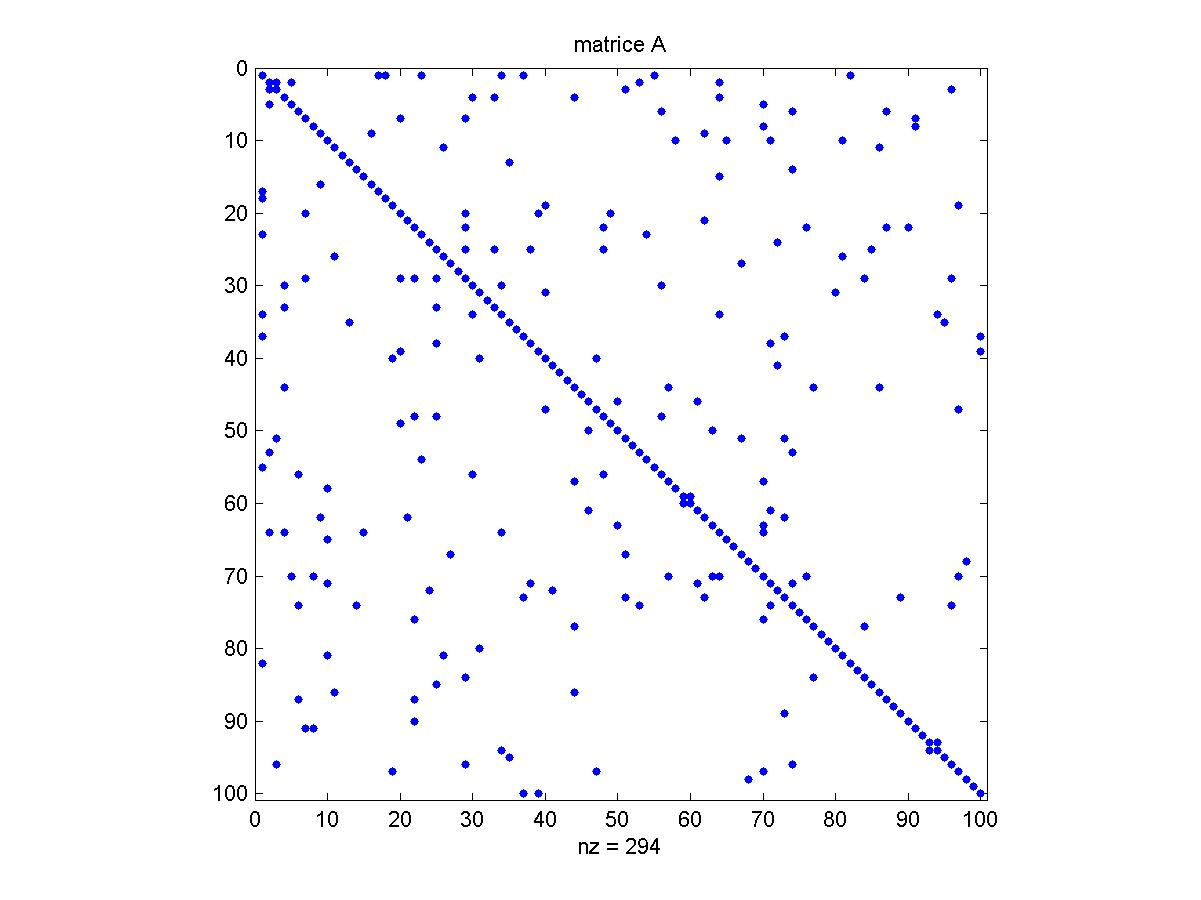
\includegraphics[width=\textwidth]{immagini/sparse.png}
    \caption{Una matrice sparsa}
\end{figure}
\begin{multicols*}{2}
Linear Algebric Representation (d'ora in avanti LAR) LAR è uno schema di rappresentazione generale per la modellazione geometrica e topologica (vedi "Rappresentazione algebrica lineare per strutture topologiche"). Il dominio dello schema è fornito da complessi cellulari mentre il suo codominio è un insieme di matrici sparse. Altro non è che un package scritto in linguaggio Julia per il calcolo geometrico di figure piane e solide.
Essa fa uso della API (Application Programming Interface) \href{https://github.com/cvdlab/ViewerGL.jl}{ViewerGL}, sviluppato dalla nostra università da una fork di \href{https://github.com/plasm-language/pyplasm/tree/master/src/plasm.jl}{Plasm.jl}.
\section{Matrici Sparse}
Nell'analisi numerica e nel calcolo scientifico, una matrice sparsa o un array sparso è una matrice in cui la maggior parte degli elementi è zero.  Non esiste una definizione rigida per quanto riguarda la proporzione di elementi con valore zero affinché una matrice si qualifichi come sparsa, ma un criterio comune è che il numero di elementi diversi da zero è all'incirca uguale al numero di righe o colonne. Al contrario, se la maggior parte degli elementi è diversa da zero, la matrice è considerata densa.  Il numero di elementi di valore zero diviso per il numero totale di elementi (ad esempio, m × n per una matrice m × n) è talvolta indicato come la scarsità della matrice.
\section{Complessi di Celle}
Una cella n-dimensionale chiusa è uno spazio topologico che è omeomorfo ad una palla chiusa n-dimensionale. Per esempio, un simplesso è una cella chiusa, e più in generale, un politopo convesso è una cella chiusa. Una cella n-dimensionale aperta è uno spazio topologico omeomorfo alla palla aperta n-dimensionale. Una cella 0-dimensionale aperta (e chiusa) è un punto.
Informalmente, un complesso di celle è uno spazio topologico ottenuto incollando fra loro un certo numero di celle chiuse. Formalmente, un complesso di celle è uno spazio di Hausdorff \textbf{$\chi$} dotato di una partizione in celle aperte (di dimensioni variabili) che soddisfa due proprietà:\begin{enumerate}
    \item Per ogni cella n-dimensionale aperta C nella partizione di X, esiste una mappa continua f della palla n-dimensionale chiusa su X tale che\begin{itemize}
        \item la restrizione di f all'interno della palla chiusa è un omeomorfismo sulla cella C, e
        \item l'immagine del contorno della palla chiusa è contenuta nell'unione di un numero finito di celle aventi tutte dimensione inferiore ad n.
    \end{itemize}
    \item Un sottoinsieme di X è chiuso se e soltanto se incontra la chiusura di ciascuna cella in un insieme chiuso.
\end{enumerate}
Il termine CW-complesso, mutuato dall'inglese, è a volte usato come sinonimo di complesso di celle. Le lettere C e W indicano i termini inglesi closure-finite e weak-topology e si riferiscono alle due proprietà elencate (la seconda proprietà infatti indica che la topologia su X è in un certo senso una topologia debole).
\end{multicols*}
\chapter{Stato dell'arte}
\begin{figure}[!h]
    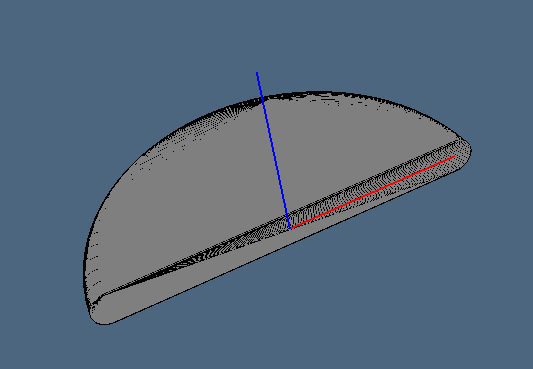
\includegraphics[width=\textwidth]{./immagini/mapperJL1.png}
    \caption{Visualizzazione grafica della funzione "pizza"}
\end{figure}
\begin{multicols*}{2}
Nel momento in cui abbiamo preso in mano questo progetto, esso si presentava
con pochi difetti in realtà. Al di là di qualche problema di configurazione
iniziale dovuta a delle dipendenze Julia non soddisfatte, infatti, l'unico 
intervento necessario era quello di ottimizzare i tempi di esecuzione.
Non erano quindi presenti errori veri e propri nel codice, ma il nostro obbiettivo
era quello di migliorare le prestazioni del programma.
\section{Mapper.jl}
L'obbiettivo primario del file mapper.jl contiene l'implementazione di diverse primitive parametriche, incluse curve, superfici e solidi incorporati in 2D o 3D.
L'approccio costruttivo è comune a tutti i metodi. Consiste nel generare una scomposizione semplice o cuboidale di un semplice dominio geometrico in
u,v o u,v,w spazio parametrico. Quindi un cambio di coordinate, ad es. da coordinate cartesiane a coordinate polari o cilindriche, si applica ai vertici della cellula
complesso che decompone il dominio.\\
LinearAlgebricRepresentation, come il suo linguaggio geometrico antenato PLASM e la sua libreria padre pyplasm mira ad essere multidimensionale. Quindi
alcune funzioni generano modelli geometrici di dimensioni variabili. Esempi importanti sono cuboidGrid e simplexGrid, il cui parametro unico è
la forma della mesh generata, ovvero il numero di celle $d$-dimensionali in ciascuna dimensione, con d = lunghezza(forma). I vertici della mesh rimangono
sulla griglia intera di dimensioni e dimensioni adeguate.\end{multicols*}
\begin{figure}[!h]
    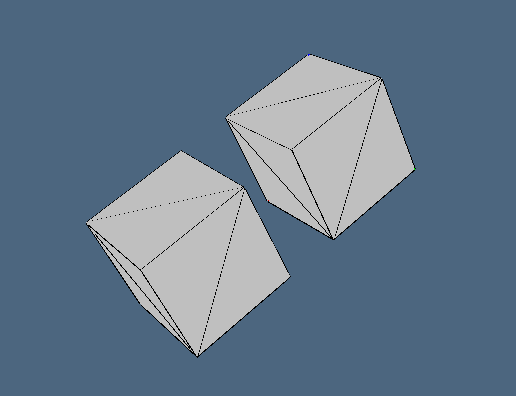
\includegraphics[width=\textwidth]{./immagini/mapperJL2.png}
    \caption{Una Visualizzazione grafica di due cubi tramite ViewerGL}
\end{figure}
\begin{multicols*}{2}
\chapter{Background Tecnologico}
In questo progetto abbiamo fatto uso di diverse tecnologie, a partire dal linguaggio Julia, utilizzato per implementare tutto quanto, passando poi per gli elementi principali della programmazione,
come i task, il multithreading e infine implementando tutto in modo tale da sfruttare la potenza di calcolo di una GPU NVidia.
\section{Julia}
Julia è un linguaggio di programmazione dinamico di alto livello, ad alte prestazioni. Sebbene sia un linguaggio generico e possa essere utilizzato per scrivere qualsiasi applicazione, molte delle sue caratteristiche sono adatte per l'analisi numerica e la scienza computazionale.
Aspetti distintivi del design di Julia includono un sistema di tipi con polimorfismo parametrico in un linguaggio di programmazione dinamico; con invio multiplo come paradigma di programmazione principale. Julia supporta l'elaborazione simultanea, parallela (componibile) e distribuita (con o senza l'utilizzo di MPI o il corrispondente integrato ai thread "stile OpenMP") e la chiamata diretta di C e librerie Fortran senza codice colla. Julia utilizza un compilatore just-in-time (JIT) denominato "just-ahead-of-time" (JAOT) nella community di Julia, poiché Julia compila tutto il codice (per impostazione predefinita) in codice macchina prima di eseguirlo.
Julia è raccolta di rifiuti, utilizza la valutazione desiderosa e include librerie efficienti per calcoli a virgola mobile, algebra lineare, generazione di numeri casuali e corrispondenza di espressioni regolari. Sono disponibili molte librerie, incluse alcune (ad es. per trasformazioni di Fourier veloci) che erano state precedentemente fornite in bundle con Julia e ora sono separate.
Diversi strumenti di sviluppo supportano la codifica in Julia, come ambienti di sviluppo integrati (ad es. Visual Studio Code di Microsoft, con estensioni disponibili che aggiungono il supporto di Julia agli IDE, ad es. fornendo supporto per debug e linting); con strumenti integrati, ad es. un profiler (e il supporto per i grafici di fiamma disponibili per quello integrato), un debugger e il pacchetto Rebugger.jl "supporta il debug a esecuzione ripetuta" e altro ancora.
\section{Julia Artifacts}
Gli artefatti\cite{artifacts} in Julia esistono sotto forma di un modulo all'interno del modulo Pkg chiamato Pkg.Artifacts. Si accede alla funzionalità nel REPL tramite:
\begin{verbatim}
 julia> using Pkg.Artifacts    
\end{verbatim}
Se inserire immagini, file binari, set di dati e dati simili nei repository git fosse indolore e senza problemi, potremmo non aver bisogno di Artifacts.\\
Il problema è che per i file binari i requisiti di spazio possono diventare eccessivi abbastanza rapidamente.
Compilare una versione per ogni piattaforma, 32-bit, 64-bit e una moltitudine di altre varianti e mantenerla nella libreria del codice sorgente è una pratica troppo onerosa: ci vorrebbe troppo spazio.\\
Con Artifacts, più pacchetti potrebbero in linea di principio utilizzare gli stessi dati e non è necessario scaricarli due volte. Facciamo conto che il pacchetto A e il pacchetto B, entrambi dipendono dalla libreria Qt. La soluzione fittizia a questo è che entrambe le librerie memorizzino una copia di Qt.\\
Bisognerebbe quindi scaricare un'enorme libreria due volte sprecando il doppio dello spazio sul disco rigido. Non è una buona soluzione. Ora qualcun altro potrebbe pensare di essere intelligente e archiviare Qt in una directory condivisa per entrambi i pacchetti da usare. Vari sistemi operativi lo hanno fatto all'inizio e hanno creato la cosa divertente che chiamiamo "inferno DLL". Ciò accade quando la versione Qt richiesta non è proprio la stessa. La versione scaricabile Qt potrebbe funzionare per A, ma non per B.\\
Git ha reso popolare una soluzione a questo enigma chiamato dati indirizzabili al contenuto. Ciò significa che non localizzano i dati fornendo percorsi come \verb|A/libs/Qt|, ma usiamo invece degli hash.\\
In questo caso, ogni byte dei binari della libreria Qt viene inserito in un algoritmo di hashing e crea un numero univoco, l'hash. In teoria, ovviamente, non è possibile garantire che due set di dati producano hash diversi. La possibilità che diversi set di dati producano lo stesso hash è simile a quella di due persone in posizioni casuali sulla terra che raccolgono lo stesso granello di sabbia. Potrebbe succedere, ma è improbabile.\\
Il sistema di pacchetti Julia può quindi verificare se una libreria è stata già installata controllando se esiste già una directory con un hash ed evitare di scaricare la stessa libreria una seconda volta.
\\Un altro problema risolto con Artifacts è che si evita di gonfiare il proprio repository con file binari. Supponiamo che tu abbia un pacchetto \verb|Museo| con il codice per mostrare i \verb|quadri|. Invece di inserire una directory \verb|quadri| nel repository del pacchetto con le immagini di ogni opera d'arte, crei un file \verb|Artifacts.toml|. In esso descrivi dove si trovano le varie immagini in una maniera simile a questa:
{\small\begin{verbatim}
    # Museo/Artifacts.toml 
    [pictures]
    git-tree-sha1 = "c5f4d31e5c9c5d6fba2469ceff3d9916050d92d2"
    lazy = true

    [[pictures.download]]
    sha256 = "2aea399ab3c6b6e3a4285ec6ae31b858803442bf1b3e3e4889a2e3e8287d56c6"
    url = "https://github.com/johndoe/Museo.jl/releases/download/pictures.tar.gz"
\end{verbatim}}
\section{Thread}
Un thread è un singolo flusso sequenziale di controllo all'interno di un programma.~\cite{threads}\\
La vera eccitazione che circonda i thread non riguarda un singolo thread sequenziale. Piuttosto, si tratta dell'uso di più thread in esecuzione contemporaneamente ed eseguire attività diverse in un unico programma. Questo uso è illustrato nella figura successiva.
% \begin{figure}[!h]
%     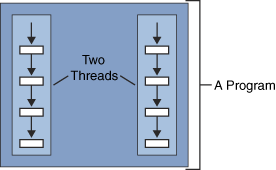
\includegraphics[width=\textwidth]{immagini/threads.png}
% \end{figure}
\\Un browser Web è un esempio di applicazione multithread. All'interno di un browser tipico, puoi scorrere una pagina mentre sta scaricando un'applet o un'immagine, riprodurre animazioni e suoni contemporaneamente, stampare una pagina in background mentre scarichi una nuova pagina o guardare tre algoritmi di ordinamento che corrono verso il traguardo.
\\Alcuni testi chiamano un thread un processo leggero. Un thread è simile a un processo reale in quanto entrambi hanno un unico flusso sequenziale di controllo. Tuttavia, un thread è considerato leggero perché viene eseguito nel contesto di un programma completo e sfrutta le risorse allocate per quel programma e l'ambiente del programma.
\\\\\\\\\\\\\\\\\\\\\\\\\
\section{Tasks}
Una coroutine o task è simile a un thread: è una linea di esecuzione, con il proprio stack, le proprie variabili locali e il proprio
puntatore alle istruzioni; il tutto però è condiviso con altre coroutine. La principale differenza tra thread e coroutine è che,
concettualmente (o letteralmente, in una macchina multiprocessore), un programma con thread esegue diversi thread in parallelo. 
Le coroutine, d'altra parte, sono collaborative: in un dato momento, un programma con coroutine esegue solo una delle sue coroutine
e questa coroutine in esecuzione sospende la sua esecuzione solo quando richiede esplicitamente di essere sospesa.~\cite{tasks}\\
L'istruzione 'yield' in Julia ha lo scopo di creare coroutine. Quando si incontra l'istruzione 'yield', lo stato corrente della
funzione viene salvato e il controllo viene restituito alla funzione chiamante.
La funzione chiamante può quindi ritrasferire l'esecuzione alla funzione cedente e il suo stato verrà ripristinato al punto in cui
è stato riscontrato lo 'yield' e l'esecuzione continuerà.
\section{Architettura Tesla}
Tesla è il nome in codice di una microarchitettura GPU sviluppata da Nvidia e rilasciata nel 2006, come successore della microarchitettura Curie. Prende il nome dal pioniere dell'ingegnere elettrico Nikola Tesla. Come prima microarchitettura di Nvidia a implementare gli shader unificati, è stata utilizzata con GeForce serie 8, GeForce serie 9, serie GeForce 100, serie GeForce 200 e serie GeForce 300 di GPU prodotte collettivamente in 90 nm, 80 nm, 65 nm, 55 nm, e 40 nm. Era anche nella GeForce 405 e nei moduli di elaborazione Quadro FX, Quadro x000, Quadro NVS e Nvidia Tesla.
Tesla ha sostituito le vecchie microarchitetture a pipeline fissa, rappresentate al momento dell'introduzione dalla serie GeForce 7. Ha gareggiato direttamente con la prima microarchitettura shader unificata di AMD denominata TeraScale, uno sviluppo del lavoro di ATI su Xbox 360 che utilizzava un design simile. Tesla è stato seguito da Fermi.
\end{multicols*}
\begin{figure}[!h]
    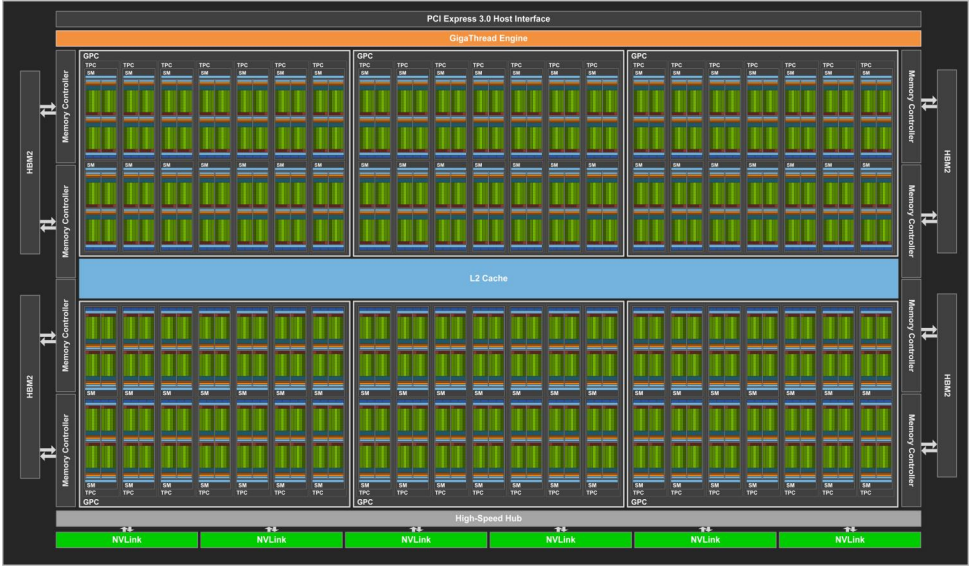
\includegraphics[width=\textwidth]{immagini/Schermata del 2022-06-23 11-33-59.png}
    \caption{Architettura Tesla di GPU Nvidia}
\end{figure}
\begin{multicols*}{2}
\chapter{Applicazione Pratica}
\chapter{Conclusioni e Sviluppi Futuri}
I benchmark eseguiti e i test effettuati sulla versione finale del progetto riportano risultati incoraggianti, i quali sono riportati di seguito.

Compito di chi verrà dopo di noi sarà quello di sfruttare questa libreria per un calcolo geometrico veloce ed ottimizzato, con la speranza che il nostro lavoro venga messo a servizio di grandi realtà.
\end{multicols*}
\normalsize
\bibliography{sitografia}
\end{document}